% ------------------------------------------------------------------------------
% TYPO3 CMS 8.1 - What's New (English Version)
%
% @author	Patrick Lobacher <patrick@lobacher.de> and Michael Schams <schams.net>
% @license	Creative Commons BY-NC-SA 3.0
% @link		http://typo3.org/download/release-notes/whats-new/
% @language	English
% ------------------------------------------------------------------------------
% LTXE-CHAPTER-UID:		dcfe6009-2200ad81-816c2edb-1f54c687
% LTXE-CHAPTER-NAME:	Backend User Interface
% ------------------------------------------------------------------------------

\section{Backend User Interface}
\begin{frame}[fragile]
	\frametitle{Backend User Interface}

	\begin{center}\huge{Chapter 1:}\end{center}
	\begin{center}\huge{\color{typo3darkgrey}\textbf{Backend User Interface}}\end{center}

\end{frame}

% ------------------------------------------------------------------------------
% LTXE-SLIDE-START
% LTXE-SLIDE-UID:		5d3d70fa-92a2935e-f1cbdc1e-285ec842
% LTXE-SLIDE-TITLE:		Feature: #75497 - inline backend layout wizard
% LTXE-SLIDE-REFERENCE:	!Feature-75497-InlineBackendLayoutWizard.rst
% ------------------------------------------------------------------------------
\begin{frame}[fragile]
	\frametitle{Backend User Interface}
	\framesubtitle{Inline Backend Layout Wizard}

	A new render type has been added to render the backend layout wizard inline in FormEngine
	(in TCA: \texttt{'renderType' => 'belayoutwizard'}).

	\begin{figure}
		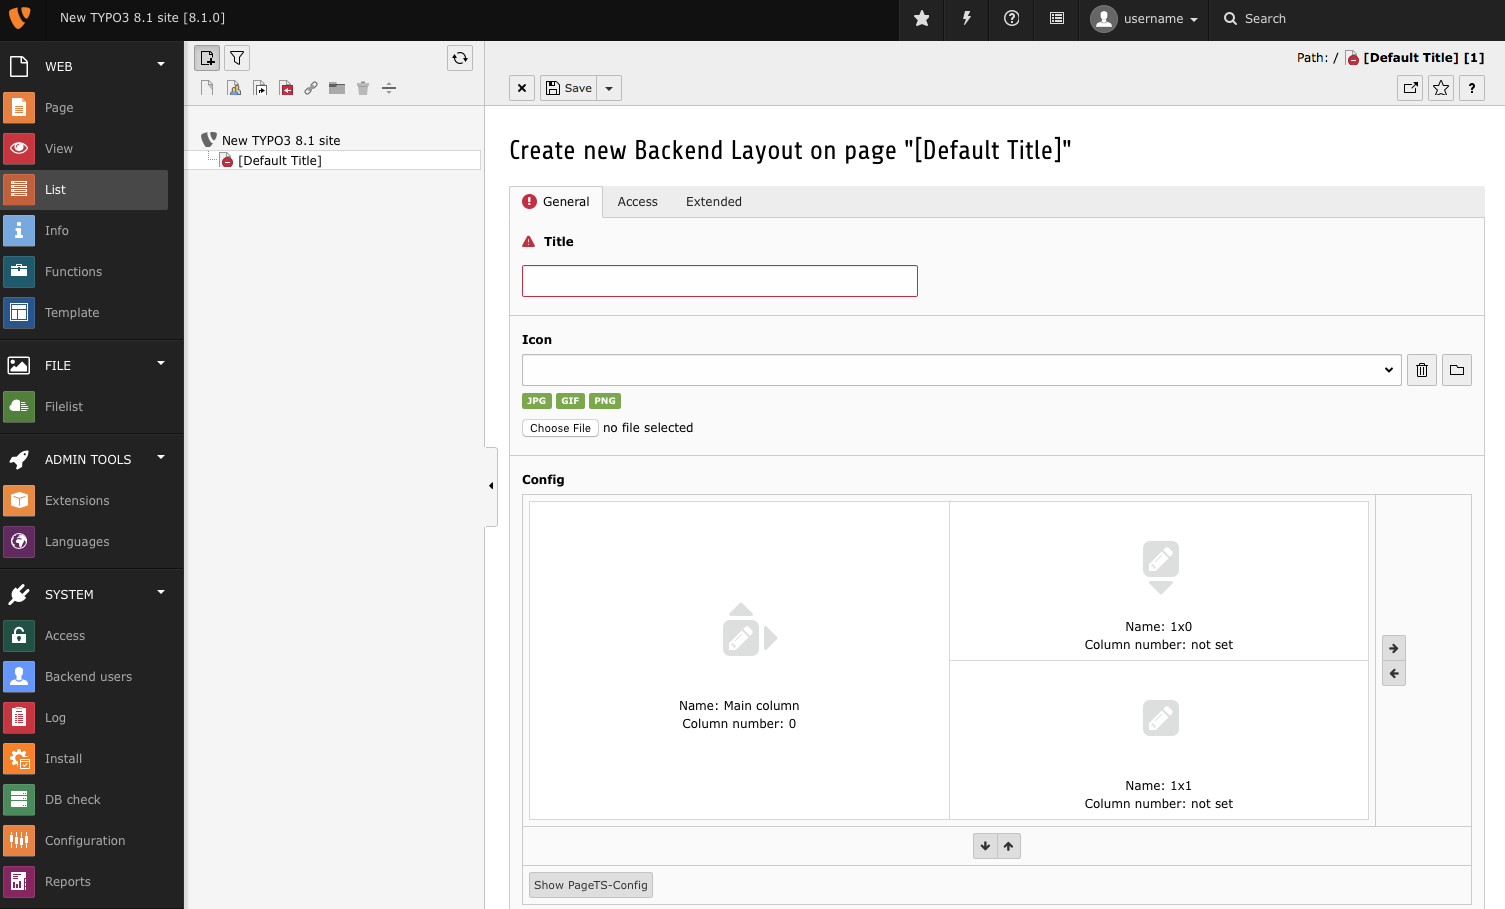
\includegraphics[width=0.70\linewidth]{BackendUserInterface/75497.png}
	\end{figure}

\end{frame}


% ------------------------------------------------------------------------------
% LTXE-SLIDE-START
% LTXE-SLIDE-UID:		7cab4dc0-cdfe9472-a3f0a874-dddf137d
% LTXE-SLIDE-TITLE:		Feature: #75581 - Simplify cache clearing
% LTXE-SLIDE-REFERENCE:	!Feature-75581-SimplifyCacheClearing.rst
% ------------------------------------------------------------------------------
\begin{frame}[fragile]
	\frametitle{Backend User Interface}
	\framesubtitle{Simplify Cache Clearing}

	The cache clearing system has been simplified by removing options in cache clear menu and
	Install Tool.

	\begin{itemize}

		\item \textbf{Flush frontend caches:}\newline
			\small
				Clears frontend and page-related caches, like before.
			\normalsize

		\item \textbf{Flush all caches:}\newline
			\small
				Clears all system-related caches, including the class loader, localization,
				extension configuration file caches and opcode caches. Rebuilding this cache
				may take some time.
			\normalsize

	\end{itemize}

	\begin{figure}
		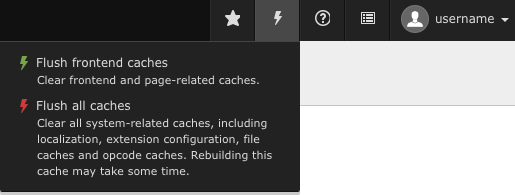
\includegraphics[width=0.45\linewidth]{BackendUserInterface/75581.png}
	\end{figure}

\end{frame}

% ------------------------------------------------------------------------------
% LTXE-SLIDE-START
% LTXE-SLIDE-UID:		e24e593c-fe9bcff9-c386db3a-79491de1
% LTXE-SLIDE-TITLE:		Rework Workspaces (1)
% LTXE-SLIDE-REFERENCE:	Rework Workspaces
% ------------------------------------------------------------------------------
\begin{frame}[fragile]
	\frametitle{Backend User Interface}
	\framesubtitle{Reworked Workspaces (1)}

	\begin{itemize}

		\item The workspace module to manage staged content has been rewritten and
			integrates much better into the visual appearance of the backend now

		\item Editors will realize straight away, it fits the overall look and feel
			due to its technical base with Twitter Bootstrap and jQuery

		\item This change also brings a performance boost and is a huge leap forward
			to a cleaner and faster TYPO3 backend with less JavaScript

	\end{itemize}

\end{frame}

% ------------------------------------------------------------------------------
% LTXE-SLIDE-START
% LTXE-SLIDE-UID:		fe9bcff9-e24e593c-79491de1-c386db3a
% LTXE-SLIDE-TITLE:		Rework Workspaces (2)
% LTXE-SLIDE-REFERENCE:	Rework Workspaces
% ------------------------------------------------------------------------------
\begin{frame}[fragile]
	\frametitle{Backend User Interface}
	\framesubtitle{Reworked Workspaces (2)}

	Screenshots of the workspace module:

	\begin{figure}
		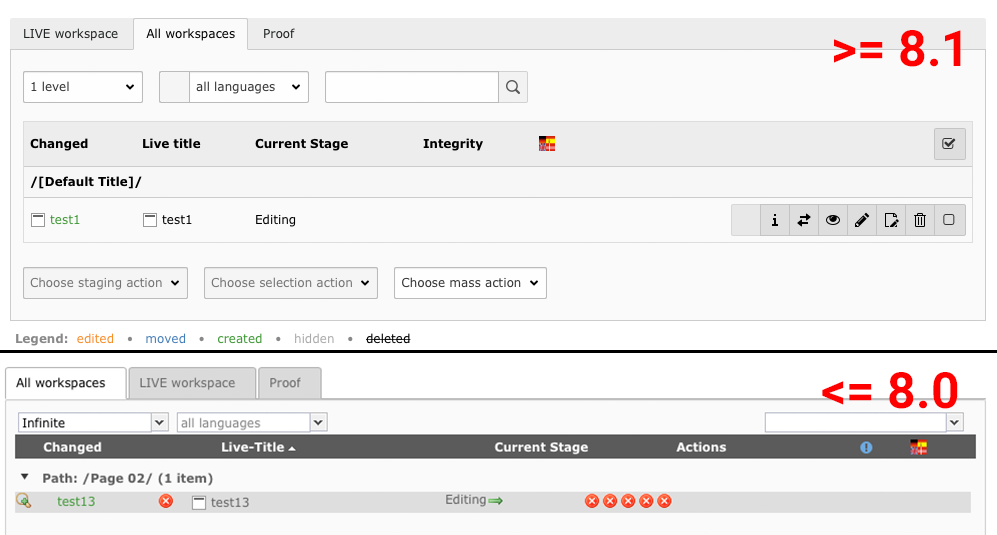
\includegraphics[width=0.85\linewidth]{BackendUserInterface/workspaces.png}
	\end{figure}

\end{frame}

% ------------------------------------------------------------------------------
